\chapter{Onderzoek: Methode en tooling voor SOUP-analyses binnen Eaglescience}\label{ch:onderzoek-tool-methode}
In het vorige hoofdstuk is duidelijk geworden dat er veel externe bibliotheken worden gebruikt bij de ontwikkeling van applicaties. Veel bedrijven kunnen niet meer zonder en Eaglescience is hier geen uitzondering op. Het gebruik van externe bibliotheken biedt namelijk veel voordelen op het gebied van besparing (tijd en geld), flexibiliteit en standaardisering, ten opzichte van interne ontwikkelde bibliotheken. Het gebruik van externe bibliotheken is echter niet zonder gevaren. Het is daarom zaak om, volgens de OWASP aangegeven manier, te controleren wat de staat is van de te gebruiken bibliotheken. Als dit niet gedaan wordt, bestaat de kans dat informatie wordt bemachtig of dat functionaliteit binnen een applicatie misbruikt kan worden door kwaadwillenden. Er bestaan bronnen zoals de NVD van het NIST waarin deze kwetsbaarheden worden opgeslagen. Het is echter ondoenlijk om deze database met de hand te doorzoeken. Zeker op het moment dat applicaties dusdanig veel bibliotheken gebruiken dat het volume simpelweg te groot wordt. Volgens de aanwijzingen van OWASP\-top10 dienen alle dependencies en de geneste dependencies gecontrolleert te worden.

Dit onderzoek beoogt om tooling en methoden te identificeren voor Eaglescience om automatisch en periodiek SOUP-analyses te kunnen doen zodat kwetsbaarheden in applicaties inzichtelijk kunnen worden gemaakt. Door gebruik van deze methode hoeft alleen de applicatie nog met de hand up\-to\-date te worden gehouden. Dit laatste is door de complexiteit bewust uit de opdracht gehouden. Een bijkomend voordeel is dat er door de SOUP-analyse naast de kwetsbaarheden ook gegevens worden vastgelegd over de bibliotheken waardoor er in de toekomst een beter beeld bestaat over het gebruik daarvan. Dit beeld kan gebruikt worden om bij een gevonden kwetsbaarheid te achterhalen welke applicaties hier ook afhankelijk van zijn. Dit leverd op zijn beurt weer een directere manier van onderzoek op.

De onderzoeksvraag is: "Welke SCA tooling is compatibel met de omgeving van Eaglescience en welke methode kan worden toegepast om deze tooling te gebuiken voor het automatisch analyseren van externe dependencies?". De hoofdvraag werpt de volgende deelvragen op, verdeelt in twee domeinen, die ieders hieronder worden beantwoord in een eigen paragraaf waarna in de conclusie de methode wordt beschreven die geschikt wordt geacht als basis voor het ontwerp.
\begin{itemize}
    \item Huidige situatie binnen Eaglescience:
    \begin{itemize}
        \item Welke werkwijze en Dev\-stack gebruikt Eaglescience voor het ontwikkelen van software?
        \item Hoe wordt er op dit moment software uitgerold binnen Eaglescience?
        \item Wat zijn de selectiecriteria voor tools die gebruikt kunnen worden?
    \end{itemize}

    \item Onderzoek om de huidige situatie binnen Eaglescience om te zetten naar de nieuwe situatie:
    \begin{itemize}
        \item Welke tools zijn er beschikbaar?
        \item Hoe zijn deze tools te integreren in de huidige buildstraat van Eaglescience?
        \item Welke methode kan worden gebruikt om middels de gevonden tools informatie over kwetsbaarheden binnen externe bibliotheken te vinden?
    \end{itemize}
\end{itemize}


\section{Werkwijze en Dev-stack binnen Eaglescience}\label{sec:werkwijze-en-dev-stack-binnen-eaglescience}
Voordat er kan worden onderzocht welke tools en methode er geschikt zijn om een analyse te doen op projecten die Eaglescience in haar beheer heeft, dient er gekeken te worden naar de manier waarop Eaglescience werkt en met welke middelen projecten worden ontwikkeld. Deze kennis is nodig om een scope aan te brengen in de zoektocht naar tooling.

\subsection{Werkwijze}\label{subsec:ESwerkwijze}
Binnen Eaglescience wordt er geprobeerd om "full Scrum" te werken. Dit wil zeggen dat voor ieder project een team van maximaal 9 full-stack developers wordt aangewezen. De sprints duren ongeveer 2 á 3 weken afhankelijk van wensen van de klant en beschikbaarheid van ontwikkelaars. Iedere sprint begint met een refinement door het team waarbij de taken die op de backlog staan worden bekeken en ingeschat. Tijdens de sprint vindt de ontwikkeling, opgedeeld in taken, plaats welke vervolgens worden gereviewd door een ander teamlid. Aan het einde van de sprint vindt er een retrospective plaats en eventueel een demo om de voortgang te demonstreren aan de klant. Dit is ook het moment dat het team ziet hoe de applicatie in het algemeen werkt. Daarnaast kunnen de projectmanager en product owner de taken die op de back-log staan opnieuw prioriseren, wat mee kan worden genomen in de volgende sprint. Als laatste is dit ook het moment waarbij een uitrol wordt uitgevoerd naar acceptatie en dys ook het meest geschikte moment voor een SOUP-analyse.


\subsection{Dev-stack}\label{subsec:ESdev-stack}
Eaglescience maakt volledige full stack oplossingen. Er worden dus zowel frontend, back-end, en database oplossingen ontwikkelt binnen projecten. Hierom wordt er binnen EagleScience gebruik gemaakt van verschillende ontwikkeltalen en tooling. Hieronder staan de belangrijkste vermeld.

\subsubsection{Ontwikkeltalen en frameworks}\label{subsubsec:ontwikkeltalen-en-frameworks}
Zoals eerder beschreven ontwikkelt Eaglescience software full-stack. Er wordt dus gebruik gemaakt van talen voor de frontend en back-end. Databases worden niet meegenomen in de lijst omdat deze als complete componenten worden gezien en de analyse op SOUP in deze ook niet veel zin heeft.
\begin{itemize}
    \item \textbf{Backend} De voornamelijkste taal voor het ontwikkelen van de back-end binnen Eaglescience is Scala. Hiervoor is gekozen omdat deze taal de mogelijkheid biedt om functioneel te programmeren in de Java Virtual Machine (JVM). Hierdoor kunnen bibliotheken die geschreven zijn in talen die ook ondersteunt worden door de JVM gebruikt kunnen worden door Scala. Daarbij heeft Scala de mogelijkheid om naadloos mee te groeien met een project. Deze eigenschap komt tevens terug in de naam Scala, wat een samenraapsel is van Scalable Language. De ondersteuning voor functioneel programmeren heeft als voordeel dat de geschreven code makkelijker te testen is, wat te danken is aan het juiste gebruik van pure functies. Pure functies hebben de eigenschap deterministisch te zijn, wat wil zeggen dat iedere keer als een bepaalde input in een functie komt er altijd dezelfde output verwacht kan worden, zonder dat er side-effects plaatsvinden die de staat van een applicatie onbedoelt kunnen veranderen. Dit komt de betrouwbaarheid ten goede. Deze eigenschap maakt het mogelijk om applicaties sneller en makkelijker te testen. Binnen Eaglescience worden er in bijna alle projecten een aantal frameworks/bibliotheken gebruikt die het ontwikkelen van microservice web applicaties in Scala makkelijker maken:
    \begin{itemize}
        \item \textbf{PlayFramework 2.xx} Een web framework voor de ontwikkeling van webapplicaties in Scala. Eaglescience gebruikt dit vooral als router voor de verschillende microservices die er achterliggen.
        \item \textbf{ArchES} Een intern ontwikkeld framework die de opbouw en communicatie tussen microservices in Scala verbeterd. ArchES is geinspireerd op Apache KAFKA en werkt middels dezelfde pub -> sub principe.
    \end{itemize} Binnen Scala kan er gebruik worden gemaakt van enkele buildtools zoals Maven, Gradle en Scala Build Tool (SBT). Binnen Eaglescience wordt SBT gebruikt omdat het de defacto tool is voor Scala.
    \item {Frontend}
    Voor de frontend wordt bij Eaglescience bijna altijd gebruik gemaakt van TypeScript, een extensie op Javascript. TypeScript maakt het mogelijk om in JavaScript getypeert te programmeren wat garandeerd dat bugs en andere fouten tijdens het ontwikkelen opgemerkt worden, zodat deze niet pas tijdens run-time aan het ligt komen. Eaglescience gebruikt framework Angular het meest voor de ontwikkeling van de diverse portalen en User-interfaces. NativeScript wordt gebruikt in combinatie met Angular om Mobile apps te ontwikkelen. De reden voor het gebruik van Nativescript is dat het de mogelijkheid biedt om Angular te gebruiken voor de ontwikkeling van zowel android als IOS apps. Beide ontwikkelframeworks draaien in JavaScript en om die reden wordt Node.js gebruikt als ontwikkelomgeving. Gezien JavaScript niet gecompileerd en dus niet gebuild wordt (zoals in Scala) is er alleen een voorziening voor dependency management in de vorm van Yarn en Node Package Manager (NPM). Binnen Eaglescience wordt NPM gebruikt voor het beheer van dependencies in een project.
\end{itemize}

#todo NOTE: dependency declaraties toe voegen?

\subsubsection{Tooling}\label{subsubsec:tooling}
Naast ontwikkeltalen gebruikt Eaglescience een aantal tools om dagelijkse werkzaamheden te stroomlijnen en software uit te rollen voor de klant. De tools zijn ieders verantwoordelijk voor een specifieke taak en alle projecten dienen, wanneer gepast, gebruik te maken van deze tools. Hoe de tools samenwerken en uitgerold zijn is te zien in figuur~\ref{fig:es-tooling}

\begin{itemize}
    \item \textbf{Jira}
    Binnen Eaglescience wordt Jira gebruikt voor taakbeheer binnen projecten. Hier worden taken aan projecten toegevoegd welke vervolgens in een sprint worden opgenomen. Ook de sprints worden beheerd middels Jira.
    \item \textbf{Confluence}
    Confluence wordt gebruikt voor de documentatie van de verschillende projecten waar Eaglescience aan werkt. Confluence en Jira zijn beiden van Atlassian waardoor deze met elkaar kunnen communiceren, wat op zijn beurt de documentatie vereenvoudigd. Op dit moment lijkt het erop dat Confluence een end of life heeft in 2023 en dat er hierdoor dus een vervanging moet worden gevonden.
    \item \textbf{GitLab}
    Gitlab wordt binnen Eaglescience gebruikt als Version control systeem. Er is gekozen om GitLab on premise te gebruiken op een server in eigen beheer op locatie. Gitlab biedt naast version control ook andere tooling aan die het mogelijk maken om vanuit GitLab te builden en/of uit te rollen, echter wordt dit binnen Eaglescience gedaan middels een andere tool genaamd Jenkins.
    \item \textbf{Jenkins}
    Jenkins is een open-source automation server die door Eaglescience gebruikt wordt om projecten te builden, testen, en deployen. Jenkins is gebouwd op een Java omgeving en is daarom uitermate geschikt om met gradle, Maven en SBT-projecten om te gaan. Daarnaast kan het middels diverse Shellscripts (Bash, SH, PowerShell) aanverwante taken uitvoeren. Als laatst kan het middels plugins ook uitrollen op cloud omgevingen. Om deze redenenen heeft Eaglescience gekozen om Jenkins te gebruiken. In een sectie hieronder wordt uitvoerig uitgewijd over hoe Jenkins binnen Eaglescience een project build, test en uitrold.
    \item \textbf{Portal}
    Eaglescience ontwikkeld momenteel een medewerkers portal welke tools en gegevens aan kan bieden die niet project specifiek zijn. Op dit moment wordt er een LDAP password reset tool en verlof inzage en aanvraag aangebonden. Er wordt naast de module voor SOUP-analyses ook een module ontwikkeld welke het mogelijk maakt om uren te registreren. Deze ontwikkelingen zijn een antwoord op de wens om systemen samen te voegen om zo een overzichtelijker geheel aan te kunnen bieden aan werknemers.

    \begin{figure}
        \centering
        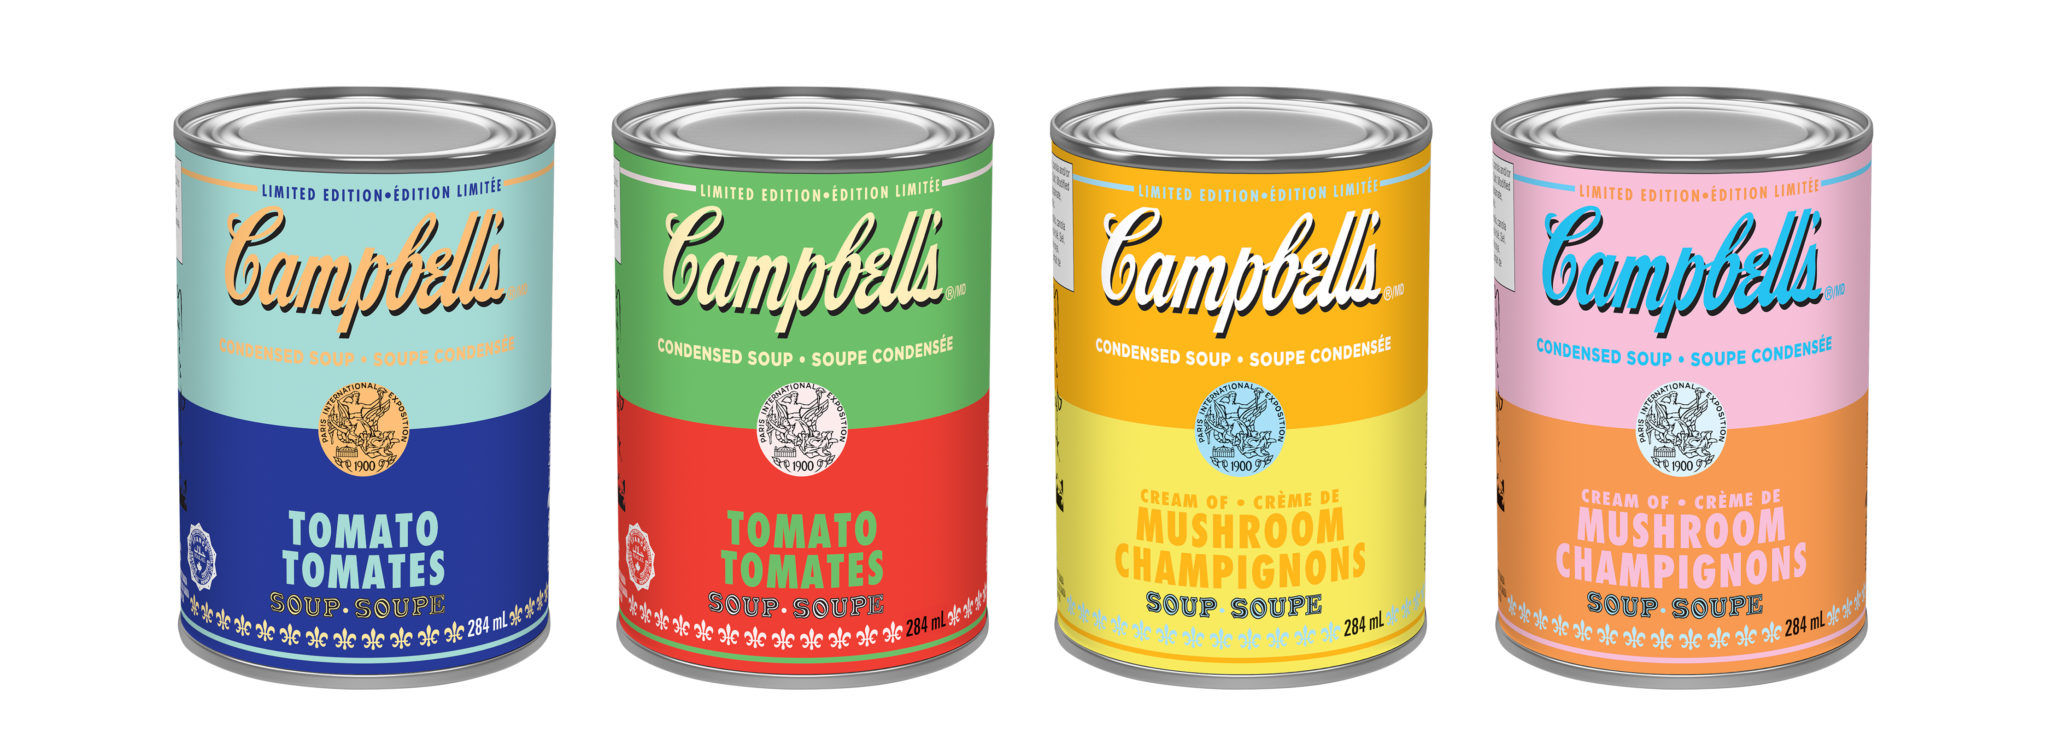
\includegraphics[width=10cm]{gfx/soupcans}
        \caption{Samenwerking van tooling binnen Eaglescience}
        \label{fig:es-tooling}
    \end{figure}

\end{itemize}


\section{Hoe wordt op dit moment software gedeployed?} \label{sec:hoe-wordt-op-dit-moment-software-gedeployed?}
Zoals hierboven is beschreven, wordt Jenkins gebruikt om de software te deployen. Het heeft de mogelijkheid om meerdere builds te doen voor verschillende projecten. Ieder project wordt op een eigen node gebouwd, waarbij de personal builds gehost worden op deze node. De development, en productie deploys gaan naar Azure in een specifiek ingerichte cluster voor deze omgevingen.

Een deploy wordt gedaan op het moment dat er source code naar GitLab gepushed wordt. Door middel van Tokens in de commit message kan gestuurd worden waar de build (als deze slaagt) gedeployed wordt bijv: {-all + portal} build en deployed alleen de portal. [ci-skip] zorgt ervoor dat er alleen een push wordt gedaan en geen build wordt gestart.
Samengevat worden er dus parameters meegegeven in de commit op basis waarvan wordt besloten of er een build moet plaatsvinden en zo ja waar en voor welke delen van de applicatie. Op deze manier wordt er flexibiliteit aan de ontwikkelaar geboden.

Een build en deploy gaat volgens de onderstaande afbeelding:

\begin{figure}[H]
    \myfloatalign
    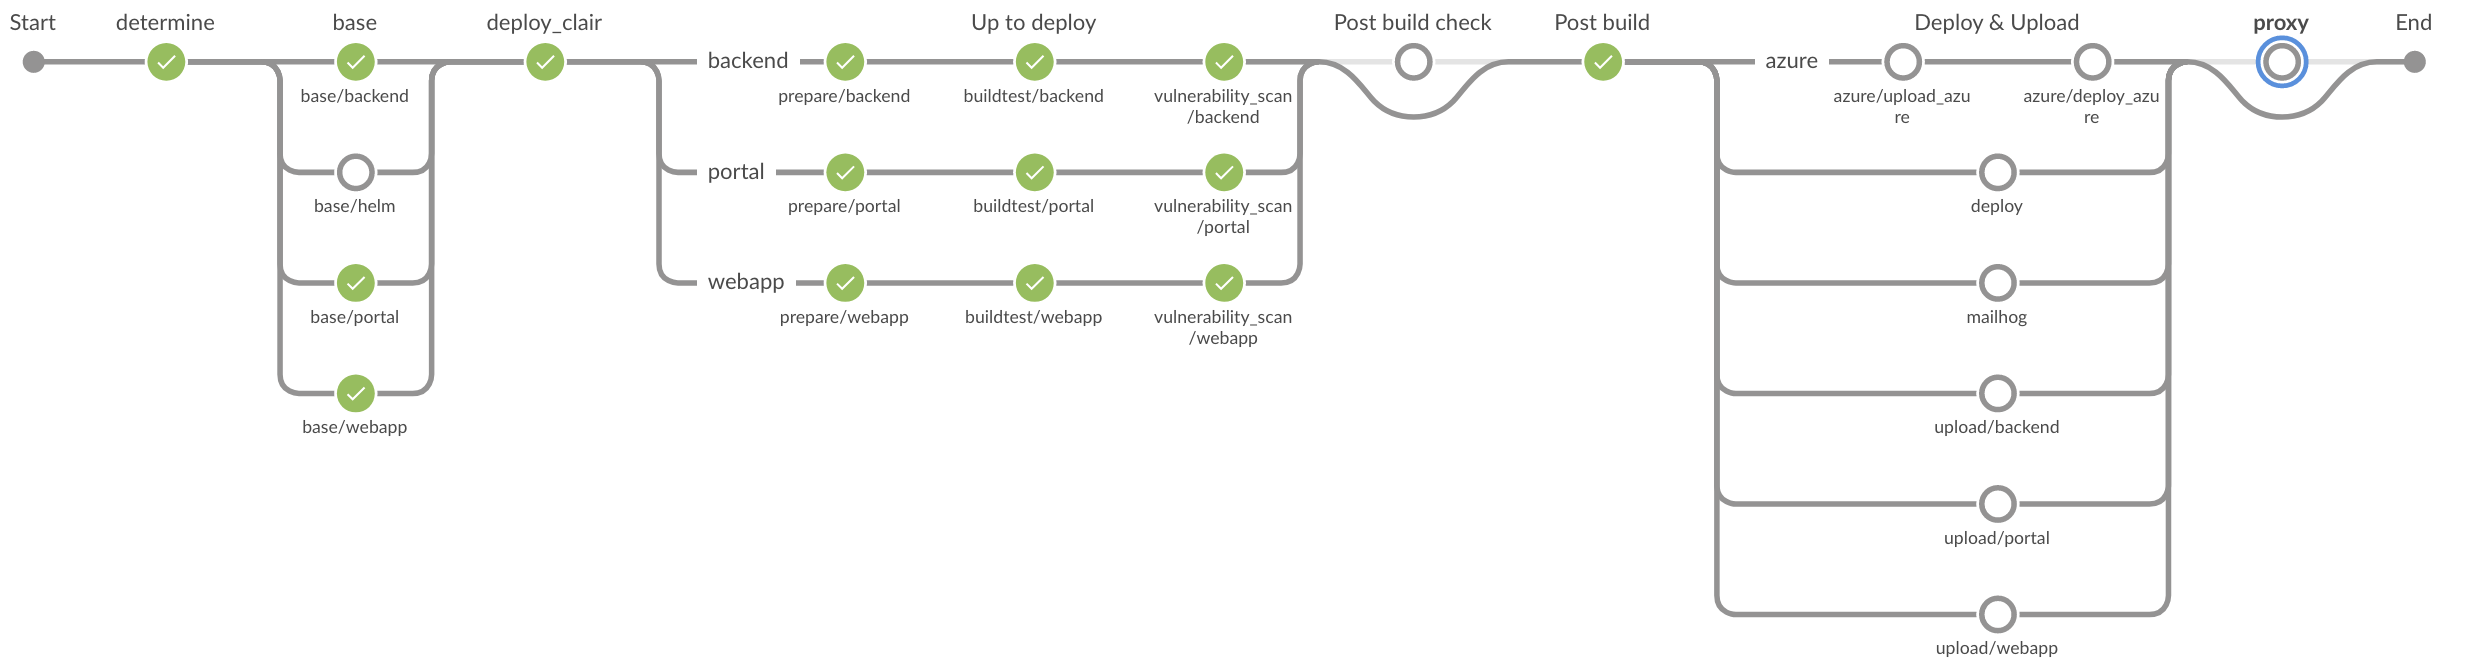
\includegraphics[width=15cm]{gfx/Screenshot 2021-08-18 Jenkins PipeLine}
    \caption{Jenkins(Blue Ocean) pipeline}
    \label{fig:JenkinsPipeLine}
\end{figure}
Een Jenkins pipeline werkt in een aantal stappen die in een .jenkinsFile worden beschreven, welke meegegeven wordt in een repository. Deze JenkinsFile wordt in de determine stap ingelezen waarna de benodigde stappen op een rij worden gezet. Hieronder worden deze stappen in meer detail beschreven:
\begin{itemize}
    \item \textbf{determine} Hier wordt bekeken,aan de hand van een JenkinsFile en tokens in de commit, welke stappen er nodig zijn om een succesvolle build en/of deploy te kunnen doen.
    \item \textbf{base} In de base stap worden alle Containers voorbereid die nodig zijn om de applicatie te builden. Images worden hier opgehaald waarna de containers worden voorbereid. De base stap is een parallel lopende stap waarin, in het voorbeeld van het figuur, backend, portal en de app worden voorbereid.
    \item \textbf{deploy clair} De clair scanner zoekt op kwetsbaarheden binnen containers die zojuist zijn aangemaakt. Dit is een extra veiligheid die ervoor zorgt dat de images en containers veilig zijn er alleen nog door bibliotheken die gebruikt worden voor ontwikkeling kwetsbaarheden kunnen worden toegevoegd.
    \item \textbf{Up to deploy}
    In het voorbeeld van het figuur wordt er voor de backend, portal, en app een parallel process gestart waarin de volgende drie substappen worden doorlopen:
    \begin{itemize}
        \item \textbf{prepare} Docker containers worden ingesteld en klaar gezet voor het ontvangen van de services.
        \item \textbf{builtest} De services worden gebuild en getest in deze stap. Eaglescience heeft een aantal tresholds opgesteld waaraan tests moeten voldoen. Om deze te analyseren worden de test resultaten vanuit de docker containers gekopieerd naar de Jenkins Store waar Jenkins de waarden kan analyseren. Als alle tests binnen de resultaten vallen wordt de volgende stap uitgevoerd.
        \item \textbf{vulnerability scan} Clair scanner scant nu de containers nogmaals, maar nu op de in de applicatie benodigde software (run time environments, databases etc.). Als clair iets vindt dat Eaglescience als verdacht acht dan wordt de build gestaakt.
    \end{itemize}
    \item \textbf{PostBuild(check)}
    Alle bevindingen worden hier gecheckt en mocht er iets mis zijn wordt er wederom afgebroken en is de build gefaald en zal er dus geen deploy plaatsvinden.
    \item \textbf{Deploy \& Upload}
    In het voorbeeld opgenomen in het figuur wordt de deploy niet uitgevoerd. Deze stap zorgt ervoor dat de gebouwde containers worden overgedragen naar Azure. Iedere container heeft wederom zijn eigen stappen. De upload valt echter buiten de scope van dit onderzoek.
    \item \textbf{End}
    Einde van de PipeLine Jenkins geeft de workers die het project heeft gebruikt weer vrij.
\end{itemize}

\section{Passende SCA tooling}\label{sec:sca-tooling}

In de opdracht staat vermeld dat de te ontwikkelen module eenvoudig in gebruik dient te kunnen worden genomen binnen de bestaande CI/CD Pipeline en dat de resultaten zichtbaar moeten zijn in de huidige portal. Hierom moet er dus Software Composition Analysis (SCA) tooling gevonden worden die makkelijk te integreren is in de huidige Jenkins pipeline, welke resultaten geeft die vervolgens te verwerken zijn tot een leesbare pagina in de portal. Als we deze stelling ontleden moeten er een aantal zaken worden onderzocht:
\begin{itemize}
    \item Welke tooling is er beschikbaar om SOUP-analyses uit te voeren op zowel SBT (Scala) als NPM (Node.js)-projecten?
    \item Welke resultaten worden er door de tool geproduceerd?
    \item Hoe kan de tooling worden geintegreerd in de huidige Jenkins pipeline?
\end{itemize}
Om deze vragen te beantwoorden moet er eerst geschikte tooling gevonden worden die, bij voorkeur, met zowel SBT als NPM-projecten overweg kan. Vervolgens dient er gekeken te worden naar hoe de geselecteerde tooling een resultaat bouwen, hoe deze eruit ziet en in welke tijd het resultaat gegeven kan worden.

\subsection{Tooling: Welke tooling is er beschikbaar om SOUP-analyses uit te voeren op zowel SBT (Scala) als NPM (Node.js)-projecten?}\label{subsec:ESTooling}
Er zijn een aantal bedrijven en instanties die tooling aanbieden om analyses te doen. Een google search op "Scala dependency scan" levert op de eerste resultaten pagina direct Snyk.io, SonarSource en OWASP op.

Snyk is een tool die geschikt is om Scala en TypeScript code, en dus bibliotheken te analyseren. Snyk kan worden ingezet op zowel SBT als NPM-projecten. Het biedt voor de analyse van code meerdere opties. Eén van die opties is middels een CLI Tool welke rapporteert naar een Dashboard gehost door Snyk zelf. Een andere optie die Snyk aanbiedt is te scannen middels een plugin via InteliJ, welke door Eaglescience gebruikt wordt. Als laatste optie biedt Snyk een plugin voor Jenkins die te integreren is in de buildstraat van Eaglescience. De voordelen van Snyk zijn dat er een volledig pakket wordt geboden, waarbij ook nog andere veiligheidsaspecten kunnen worden gecontroleerd (zoals het scannen van zelf geschreven code). Echter, om de volledige functionaliteit van Snyk te kunnen benutten is er een licentie nodig. Het nadeel hiervan is dat dit op periodieke basis geld kost. Een ander nadeel is dat de resulaten in een eigen omgeving, welke extern gehost wordt, kan worden ingezien. Hierdoor valt deze tooling echter buiten de vooraf gestelde criteria.

SonarSource is een ander bedrijf dat tooling aanbiedt voor het analyseren van source-code. Het doet dit door in de verschillende stadia van het proces tooling aan te bieden die helpen de kwaliteit van geleverde applicaties te verhogen. Als eerste biedt het een gratis plugin aan (SonarLint) voor verschillende IDE's waarbij actief wordt gekeken naar fouten, bugs en dergelijken tijdens het schrijven van code. Op die manier wordt er gekeken of code volgens standaarden worden geschreven en er geen kwetsbaarheden worden toegevoegd. Daarnaast is er een pakket dat SonarQube heet. Dit pakket biedt de mogelijkheid aan om op verschillende momenten naar de kwaliteit en de veiligheid van de aanwezige code te kijken. Hoewel SonarQube geschikt is om Scala en Typescript code te analyseren, is de SonarLint plugin niet compatibel met Scala code, maar wel met JavaScript en TypeScript. Er zijn meerdere versies beschikbaar die elk een specifiek aantal functionaliteiten aanbieden. Zo is er een community edition, welke gratis is, die als server geinstalleerd kan worden en waar verschillende repositories kunnen worden bijgehouden. Hiernaast zijn er andere editions beschikbaar waarvoor betaald moet worden en er extra functies worden geleverd, zoals GitLab integration en dergelijke. Samengevat zijn de voordelen van SonarSource tooling dat er tijdens alle stadia van software ontwikkeling controles worden ingebouwd die de code analyseren op o.a. kwetsbaarheden. Hiernaast kan SonarQube on premise draaien. Echter, een nadeel van de SonarQube plugin is dat SBT niet zelf door SonarSource ontwikkeld wordt, en SonarLint geen ondersteuning biedt voor SBT. De incompatibiliteit met Scala maakt integratie in de Eaglescience pipeline niet voor de hand liggend.

In eerdere onderzoeken is naar boven gekomen dat de OWASP zich bezig houd met het veilig houden van geschreven software. Een van de projecten die de OWASP aanbiedt is "Dependency-check". Dit is een Software Composition Analysis (SCA) Tool die het mogelijk maakt om openbaar gemaakte kwetsbaarheden te detecteren door te kijken of er voor dependencies een Common Platform Enumeration (CPE) bestaat. Als deze CPE bestaat kan er gekeken worden of er een CVE voor bestaat en vervolgens worden weergegeven in resultaten. Als geen van beiden bekend is wordt er door de tool vanuit gegaan dat er op het moment van checken geen kwetsbaarheid gevonden is. Hoewel dit op het oog een goede tool is om SOUP te analyseren, is de in het project ontwikkelde versie niet geschikt om te scannen op SBT en NPM dependencies. Op de website van het project is echter een link naar een versie die SBT-projecten kan analyseren. Uit de NPM repository blijkt dat er een soortgelijke tool bestaat om NPM-pakketten te analyseren.

De SBT depedency check en de OWASP dependency check (scanner voor NPM) lijken op dit moment de enige voor de hand liggende tooling voor de SOUP-analyse. Beide tooling zijn gratis beschikbaar en open-source. Echter zijn dit geen op zichzelf staande tools, maar bieden ze wel de mogelijkheid om te worden geintergreerd in suits zoals Snyk en SonarQube. Het feit dat ze losse tools zijn maakt het mogelijk om deze in te zetten in de buildstraat van Eaglescience. Een ander voordeel is dat beide tooling gebruik maken van dezelfde engine.
%
%https://github.com/etnetera/owasp-dependency-check for Node.js /NPM
%https://github.com/albuch/sbt-dependency-check for SBT
%
%https://github.com/eliasgranderubio/dagda niet zelfde als OWASP maar wellicht usefull

\subsection{Testen van Tools}

Het lijkt voor de hand te liggen dat zowel de SBT-dependency-check en de OWASP-dependency-check (NPM) verantwoorde keuzes zijn om verder te onderzoeken. Echter dienen deze eerst te worden onderzocht op bruikbaarheid voordat er kan worden gedacht aan implementatie. Om de bruikbaarheid te testen zijn de volgende scenario's opgesteld die samen een idee moeten geven over de werking binnen een project en toepasbaarheid binnen een methode die in de volgende sectie zal worden onderzocht.

Er is gekozen voor twee scenario's
\begin{enumerate}
    \item \textbf{Bestaand Eaglescience Project} Om te achterhalen hoe de dependency check tools kunnen worden ingezet in projecten die op dit moment ontwikkeld en gehost worden, moeten de tools worden geintegreerd in een bestaand project. Als project is gekozen voor GroeiGids,\footnote{GroeiGids is op het moment van schrijven één van de grootste projecten waar Eaglescience aan werkt wanneer wordt gekeken naar code-volume en aantal depedencies. Het is een project in opdracht van de GGZ en biedt ouders de mogelijkheid om groei informatie van hun kinderen in op te slaan.} een van de grotere projecten waar op dit moment aan wordt gewerkt. Het project bevat zowel een frontend (NPM Angular) als een App (NPM NativeScript), evenals een uit microservice bestaande SBT-project waarbij een andere manier wordt gebruikt om dependencies te declareren. Voor GroeiGids worden dependencies in een aparte file gedeclareerd en deze worden vervolgens geimporteerd in de build.sbt. Theoretisch gezien zou dit geen probleem moeten zijn gezien SBT zelf ook gebruik maakt van deze constructie.

    \item \textbf{Alleen de dependency declaraties} Door alleen dependency declaraties te gebruiken in een test, en dus niet het volledige project, kan worden onderzocht of de geselecteerde tooling hiermee om kan gaan. Dit zou wenselijk kunnen zijn om op een ander moment een analyse uit te voeren op de verschillende projecten. Het zou op die manier ook periodieke controle op kwetsbaarheden mogelijk maken zonder dat hiervoor een heel project opgezet dient te worden inclusief source-code.
\end{enumerate}

\subsubsection{Test 1a: SBT dependency scanning in een bestaand project}
\textbf{Doel:} Onderzoek naar het gebruik van de SBT-dependency-check plugin in GroeiGids. Het gewenste resultaat is kennis over hoe de plugin wordt geconfigureerd om de gewenste output, bij voorkeur een JSON file/object, te verkrijgen.
\textbf{Methode:} Als eerste dient de SBT-dependency-check plugin te worden geinstalleerd in het project middels de documentatie van het project. Vervolgens dient de output format te worden aangepast: \texttt{dependencyCheckFormats in Global += "JSON"}
en \texttt{dependencyCheckFormats in Global += "HTML"}. HTML wordt alleen gebruikt om in de test leesbare output te verkrijgen zodat deze kan worden geverifieerd met andere bronnen. Deze rapporten die resulteren in het draaien van \texttt{SBT dependencyCheck} dienen te worden gecontrolleerd tegen een andere bron. Daarnaast dient te worden bepaald hoeveel langer de analyse duurt wanneer de database wordt geupdate.
\textbf{Resultaat:} De analyse duurt ongeveer 173 seconden inclusief het ophalen/updaten van de database. Op het moment dat de database up-to-date is duurt een analyse 87 seconden. Dit zou dus inhouden dat een deploy 3 minuten langer wanneer een SOUP-analyse wordt gedraaid.
\begin{figure}[bth]
    \myfloatalign
    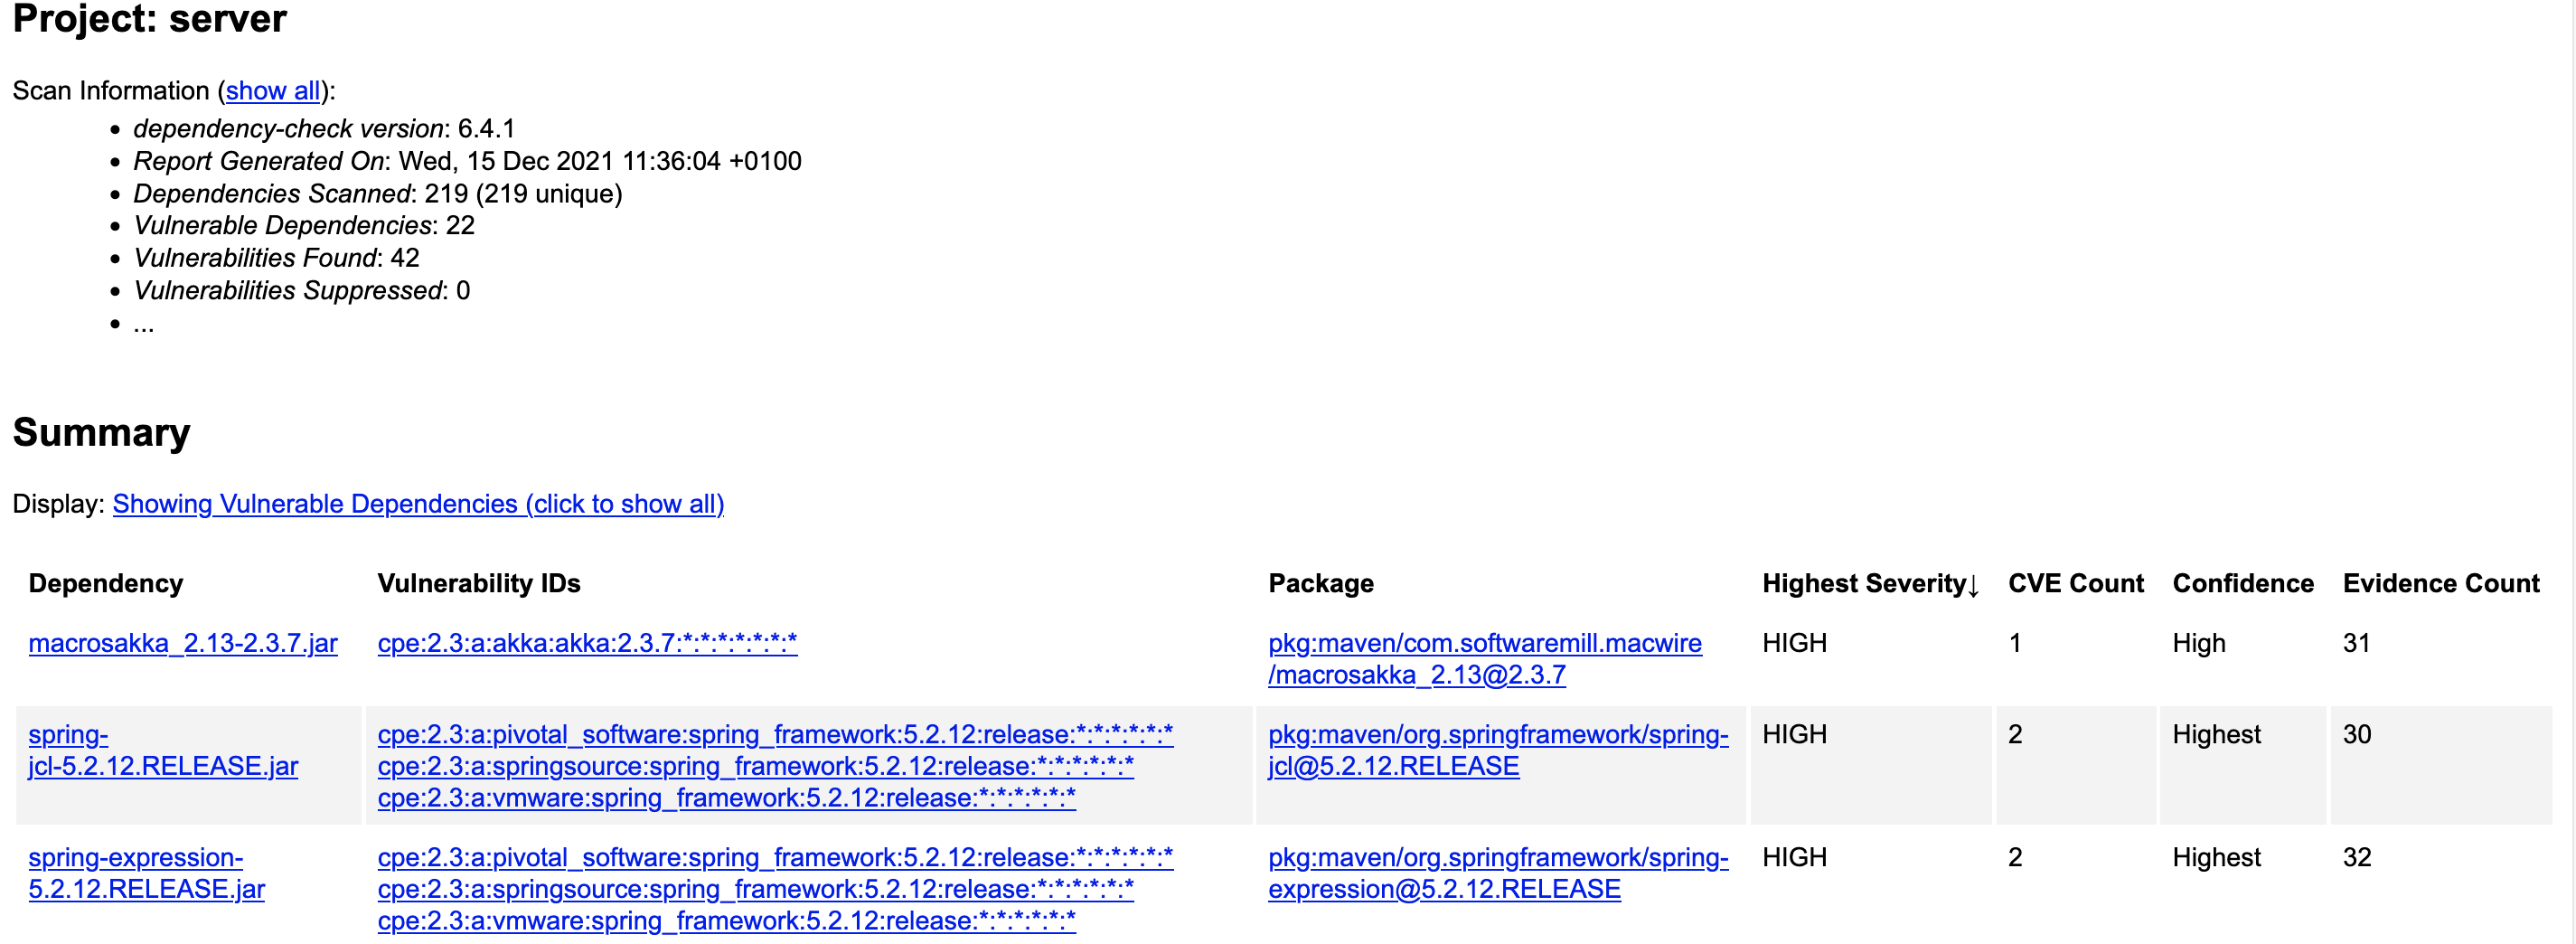
\includegraphics[width=15cm]{gfx/report_analyse_test1a_SBT}
    \caption{Deelresultaat van een analyse op de backend van groeigids}
    \label{fig:SBTReport1A}
\end{figure}

In figuur~\ref{fig:SBTReport1A} is te zien dat er 219 unieke dependencies gescanned zijn en dat er 42 kwetsbaarheden gevonden werden in 22 van de gescande dependencies. Na verificatie van de bovenste 5 vermeldingen tegen andere bronnen (opencve), bleek dat deze overeen kwamen, en het vertrouwen wordt gewekt dat de analyse correct is.

\subsubsection{Test 1b: NPM dependency scanning in een bestaand project}

\textbf{Doel:} Onderzoek naar de algemene werking van de geselecteerde plugin, waarbij vooral gekeken moet worden naar welke instellingen er relevant zijn en of de output nagenoeg overeenkomt met die van de SBT analyse. Daarnaast moet de timing worden opgenomen.
\textbf{Methode:} Voor NPM bestaat er geen plugin, welke wel beschikbaar is  voor SBT-projecten, echter wordt de OWASP-dependency-check toegevoegd als een dev-dependency \texttt{npm install -D owasp-dependency-check}, en moet er een script worden aangemaakt in package.json die het volgende aanroept \texttt{"owasp-dependency-check --project \"GroeiGids APP\" -f HTML -o \"./reports\""}. De tag HTML moet daarna vervangen worden door JSON en daarna alsnog een keer gedraait worden.
\textbf{Resultaat:} De output van deze analyse is nagenoeg gelijk aan die van de hierboven uitgevoerde analyse op SBT. De output van de check ziet er qua opmaak hetzelfde uit als die van SBT. Ook de verificatie met OpenCVE is goed dus ook hier is er het vertrouwen dat de correcte resulaten worden weergeven.


!!!! 21 sec zonder update
?? met update
weergeeft als die in de test hiervoor dat wil zeggen dat alle onderwerpen hetzelfde zijn, maar dat de inhoud dus info over de bibliotheken veranderd. Ook de beide JSON files zijn qua schema bijna identiek. Wat dus kan resulteren in een enkele procedure die de data kan omzetten naar bruikbare informatie.

\begin{figure}[bth]
    \myfloatalign
    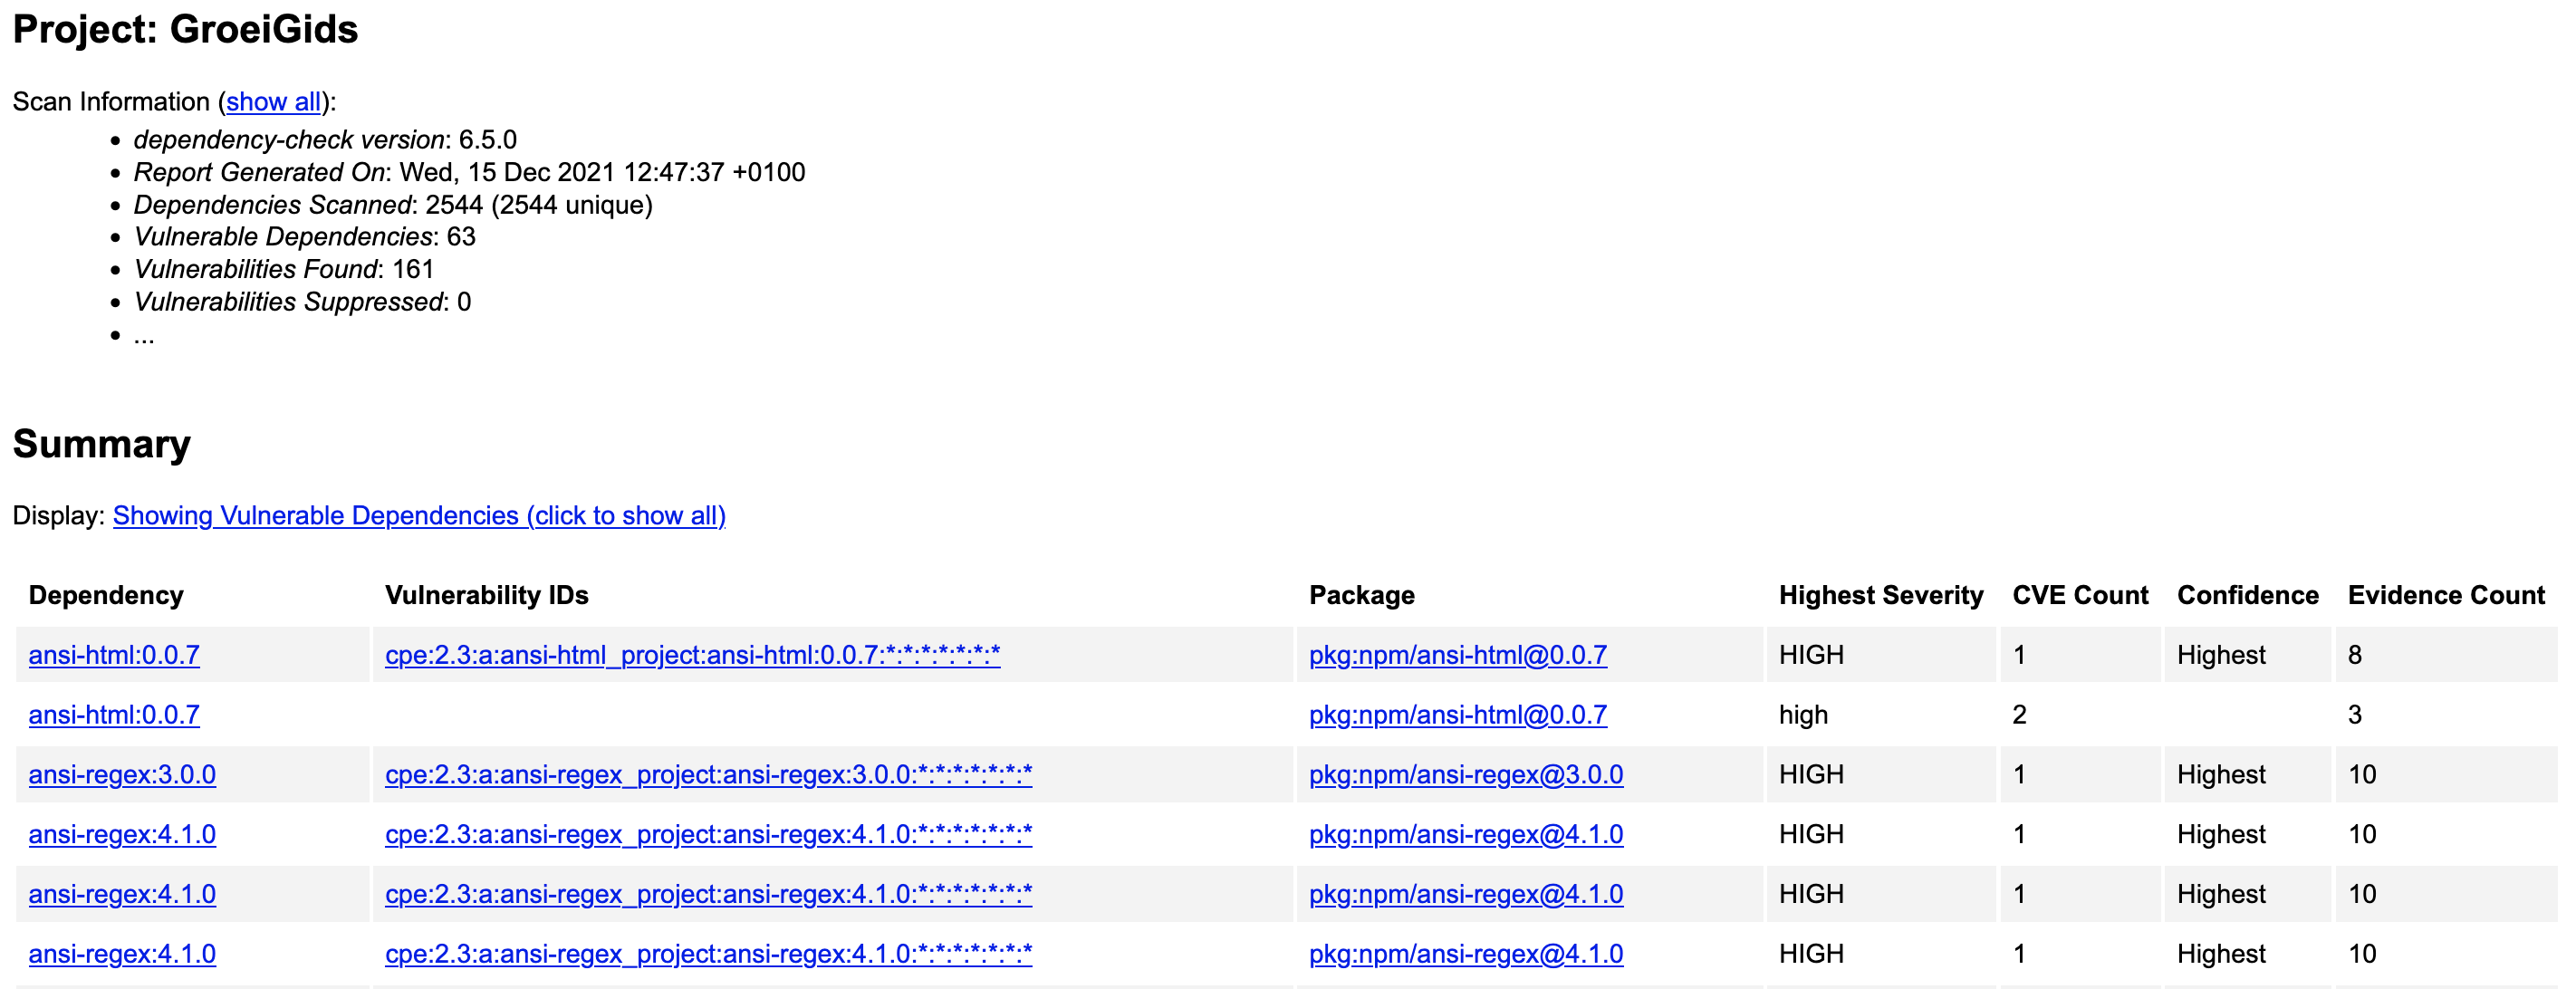
\includegraphics[width=15cm]{gfx/report_analyse_test1b_NPM}
    \caption{Deelresultaat van een analyse op de app van groeigids}
    \label{fig:SBTReport1b}
\end{figure}


\subsubsection{Test 2a: SBT alleen de dependency infomatie gebruiken.}



Om te onderzoeken of een dependency check ook uitgevoerd kan worden zonder dat er een heel project bestaat en alleen een declaratie van dependencies in de build.sbt file. De uitkomsten moeten worden op gelijkheid worden gecontroleert om op deze manier te verifieren of deze methode ook werkt.

\textbf{Doel:} Achterhalen of er verschil kan bestaan tussen analyse op een volledig project ten opzichte van een project waarvan alleen de dependencies bekend zijn.
\textbf{Methode:}Als eerst dient er een leeg sbt project gemaakt te worden waarbij

\textbf{Resultaat:}


\subsubsection{Test 2b: NPM alleen de dependency infomatie gebruiken.}
Node.js docker container opzetten..
package.json / package-lock.json copiere
npm ci
owasp script draaien
cp resulst naar buiten
destroy Container


Testen of de dependency check zonder informatie over het gebruik van de dependencies kan functioneren

\textbf{Doel:}\\ Onderzoeken of er een dependency check uitgevoerd kan worden met alleen een package.json. Onderzoeken wat er nodig is om een succesvol rapportage te verkrijgen over eventuele kwetsbaarheden en gebruik van dependencies.

\textbf{Methode:}

\begin{enumerate}
    \item Middels \texttt{NPM init} wordt er een nieuw project worden opgezet. Dit project is geheel leeg, zonder source code of dependency decalraties.
    \item Dependency check toevoegen middels \texttt{npm install -D owasp-dependency-check} en een script toevoegen die het project zal draaien: \texttt{"owasp": "owasp-dependency-check --project \" angularSandbox \" -f JSON -l\"dep-check-log.txt\" "}%TODO quotes goedzetten
    Dit meld dat er gelogt dient te worden naar dep-check-log.txt tijdens runtime en dat er een resulaat in JSON moet worden gegeneerd. ook wordt er een projectnaam meegegeven. [Checken of dit naamgeving is of daadwerkelijk functioneel].
    \item dependencies van het project groeigids toevoegen in package.json. en het owasp script wat in de vorige stap werst gedefineerd gebruiken voor een analyse en de JSON die eruit komt veilig stellen in een andere map
    \item een \texttt{npm install} uitvoeren om de dependencies te installeren in het project. Er is nog steeds geen code base op dit moment. Behalve die van de dependencies.
    \item nogmaals het owasp script draaien.
    \item JSON files met elkaar vergelijken.
\end{enumerate}

\textit{NPM init} kan gebuikt worden om een nieuwe leeg project op te zetten. hier moet vervolgens de dev-dependency-check aan toe gevoegd worden gevolgt door een \textit{NPM install}. op dit moment hebben we een leeg project met alleen de plugin geinstalleerd. vervolgens moeten de dependencies worden gekopieerd. en de check moet worden uitgevoerd. [Resultaat1] vervolgens moet er weer een \textit{NPM install} worden uitgevoerd Nu hebben we een project zonder source code en alleen de geinstalleerde dependencies. Deze dependencies dienen te worden vergeleken met de resultaten die in test 1a zijn gevonden. [Resultaat2].

\textbf{Resultaat:}\\
Het resultaat van stap 3 is dat er een analsye gedaan wordt op de package-lock.json, waar nu alleen maar een declararie staat van de dependency check. Alleen deze dependencies worden geanalyseerd en die van het project zijn niet meegenomen.


geen analyse gedaan kan worden op alleen een package.json. De tool heeft een package-lock.json nodig om in te kunnen achterhalen welke dependencies er worden gebruikt. Dit bestand wordt alleen gegenereerd op het moment dat er een \textt{npm install} wordt gedaan.
Er is een installatie nodig van de dependencies
Iedere keer wordt er een nieuwe folder aangemaakt met een nieuwe JSON dus er is geen persistence....

Daarnaast MOET er een npm install gedaan worden wil de tool deps vinden...... Dit betekend dus dat er een "npmbuild gedaan moet worden.
De NPM Dependency check voert onderwater het volgende commando uit \texttt{/dependency-check.sh --out=./dependency-check-reports --project angularSandbox -f JSON --data=/tmp/dependency-check-data --scan=package-lock.json
} de -f en de --out flags zijn de output flags wat zegt dat er een JSON file in depende-check-reports directory in de base gemaakt moet worden. --scan = package-lock.json is het bestand wat geacanned wordt wat wil zeggen dat er een node_modules folder moet zijn is aangemaakt middels een npm install op de package.json van het project. In de logs is zijn ook statements te vinden die erop wijzen dat niet geinstalleerde dependencies wordten geskipped ) \texttt{2021-12-13 15:08:36,500 org.owasp.dependencycheck.analyzer.NodePackageAnalyzer:292
WARN  - dependency skipped: node module esbuild-darwin-arm64 seems optional and not installed} Daarnaast worden de verschillen tussen de package.json en de package-lock.json niet meegenomen en is de -lock file leidend. Nog een indicatie dat er een npm install nodig is op basis van project package.json


Database opzetten voor de tool duurt een geruime tijd dus als dit in een enkele keer kan is dit al tijdswinst. Het klijkt om deze reden ook niet handig om op een deploy de analyse te runnen.


begin tool : 2021-12-13 15:01:08
eind einde opzetten benodigdheden : 2021-12-13 15:08:35
dit komt uit op 7 minuten lead time voor analyses.

andere note is dat de tool redelijk wat CPU vroeg op het moment van analyseren wat op zijn beurt de performance van het builden van andere projecten weer kan schaden./




\subsubsection{Conclusie tests:}
Een analyse voor een project zo groot als groeigids duurt in het slechtste geval ongeveer 2 minuten hierbij is geen rekening gehouden met andere taken die procesor tijd opvragen. De tijd zal oplopen op het moment dat de Jenkins Server meerdere build aan het uitvoeren is voor meerdere projecten.



Het resultaat is dat het rapport gegenereerd door de dependency-check tools nagenoeg gelijk zijn en in het JSON formaat. Uit de rapporten bleek wel dat de dependency-check engines verschilden van elkaar met een enkele major versie.

het doen van een npm install is niet optimaal omdat deze opnieuw alle dependencies uitzoekt op dependencies en mogelijke veranderingen. npm ci is een mogelijke verbetering omdat deze gebruik maakt van de lock file waarin zoals de naam doet vermoeden vast staat welke deps er gebruikt worden en de nested deps ook. dus de resolve tijd is veelkorter (https://docs.npmjs.com/cli/v8/commands/npm-ci).



%TODO METHODE
\subsection{Methode voor extractie, verwerken en het publiseren van de resultaten gevonden in de projecten van EagleScience}\label{subsec:methodeSOUPES}

\subsubsection{Methode 1: Scannen in de buildstraat}

\subsubsection{Methode 2: postponed analyseren}
Scannen op een later moment, dus door een project te bouwen op basis van een snapshot en deze op een later moment te analyseren.

\subsubsection{Resultaat:} Methode 2: het scannen op een later moment heeft de wat mij betreft de voorkeur. gezien dit de minste redundantie in datat betekend. Echter moeten er wel meer functionaliteit worden geschreven om alle processen te kunnen uitvoeren.

Beide tools generen rapporten in nagenoeg het zelfde schema. Op basis van dit schema kan een datamodel worden gegenereerd die het opslaan van de relevantie informatie. Er is ook een datamodel nodig om op te li


%\section{Conclusie}\label{sec:conclusie}
%De twee tools draaien beiden op de zelfde engine. wat er vervolgens voor zorgt dat er voor beide tools nagenoeg de zelfde output is. Echter door de complexiteit van de projecten die uitgerold worden is voor de SBT tool veel werk om alle dependencie te analyseren wat niet te goed komt in de build tijd. op basis van dit gegeven is er voor gekozen om later een analyse uit te voeren op de dependencies en de pipeline alleen de gebruikte dependencies en hun versies te borgen in een snapshot in de database en deze snapshots periodiek te analyseren op kwetsbaarheden. Het voordeel van deze manier is naast dat het minder tijd kost in de build pipeline. we de analyse kunnen uitvoeren op ieder gewenst moment en dus ook in de nachtelijke uren wanneer de servers niet de druk hebben die ze overdag hebben. Voor het ontwerp moet er dan ook een manier gevonden worden om snapshots op te slaan waarin minimaal de volgende attributen zijn vastgelegd:
%\begin{itemize}
%    \item \textbf{timestamp:} De datum en tijd wanneer de snapshot is gemaakt
%    \item \textbf{GitHash:} De Hash van de commit die de build heeft getriggered
%    \item \textbf{projectName:} Naam van het project waar de snapshot voor is gemaakt
%    \item \textbf{omgeving:} Op welke omgeving werdt er gebuild toen de snapshot is gemaakt
%    \item \textbf{projectType:} Is het een SBT of NPM project ( later uit te breiden met een MAVEN en bijv. NUGET)
%    \item \textbf{dependencyList:} Lijst van de gevonden dependencies en hun versies
%    \item \textbf{analysed:} Boolean om aan te geven of de snapshot al is geannalyseerd.
%   \item \textbf{ScalaVErsion}
% \item \textbf{SBT version}
%\end{itemize}
% Kan er worden achterhaald door middel van ene Hash of de commit nieuwer is?


%
%Voorhet maken van de snapshots moeten er in de jenkins pipeline een mechaniek worden geplaatst die de gevonden attributen kan opslaan in een database voor later gebruik.
%
%Een bijkomend voordeel van deze manier van werken is dat er een historiek onstaat in de gebruikte versies welke als bewijsvoering kan dienen bij incidenten.


\section{Methode met gekozen tooling om een analyse te doen binnen Eaglescience}\label{sec:methode}

%Todo: Toevoegen aan de conclusie van het hoofdstuk


\section{Conclusie}\label{sec:ESconclusie}
Door gebruik te maken van de werkwijze van Eaglescience en daarom tijdens elke deploy naar acceptatie en productie een snapshot op te slaan van de gebruikte bibltiotheken onstaat er een beeld in het gebruik van bibliotheken per project. Deze snapshots kunnen vervolgens worden gebruikt om op een "later" te defineren moment analyses uit te voeren op bibliotheken. Op deze manier is er


developement(TestOmgeving) of acceptatie/ productie
Binnen EagleScience wordt er gewerkt middels de SCRUM methode om software te ontwikkelen. Waarbij Jira en Confluence worden gebruikt voor de documentatie van de projecten. Het zou voor de hand kunnen liggen om informatie over de SOUP analyses in Confluence op te slaan zodat er mee gelift kan worden op dit systeem. Echter doordat de end of life van Confluence is aangekondigd dient er een alternatief worden gezocht. Welke al in de opdracht is meegenomen.

EagleScience ontwikkeld haar projecten over het algemeen in Scala en TypeScript met enkele daarbij behorende (build) tooling en wel SBT voor Scala en NPM voor node projecten. Het is dus noodzaak om voor deze twee tools en methode te vinden waarmee SOUP analyses gedaan kan worden. Daarnaast Jenkins de ideale mogelijkheid om of informatie te winnen over de staat van projecten die op dat moment uitgerold zijn. Dit kan zijn door de nog te onderzoeken methode direct door Jenkins te laten uitvoeren over door de dependency declaraties van projecten op te slaan in een omgeving waar mee extern de analyse kan woden uitvoerd.
